\section{Obligatorisk Opgave}

\subsection{Valgte fokuspunkter}

%\todo{Fokuspunkter skal godkendes} - antages godkendt
\begin{itemize}
	\item Redegør for, hvad et Software Design er.
	\item Redegør for opbygningen af Mediator Pattern.
	\item Sammenlign de forskellige variationer af GoF Mediator - hvilke bør anvendes hvornår?
	\item Sammenlign de to Design Patterns GoF Observer og GoF Mediator - hvornår vil du anvende hvilket og hvorfor?
	\item Redegør for fordele og ulemper ved anvendelsen af GoF Mediator.
	\item Redegør for hvilke(t) SOLID-princip(per) du mener anvendelsen af GoF Mediator understøtter.
\end{itemize}

\subsection{Hvad er et Software pattern?}

\derp

\subsection{Redegør for opbygningen af Mediator Pattern}
Når objekters funktionalitet distribueres ud mellem hinanden, vil der opstå høj kobling, og masser
af interkonnektivitet. I et mediator pattern oprettes et separat mediator-objekt, som står for at
kontrollere objekters interaktioner med hinanden.

\begin{figure}[H]
	\centering
	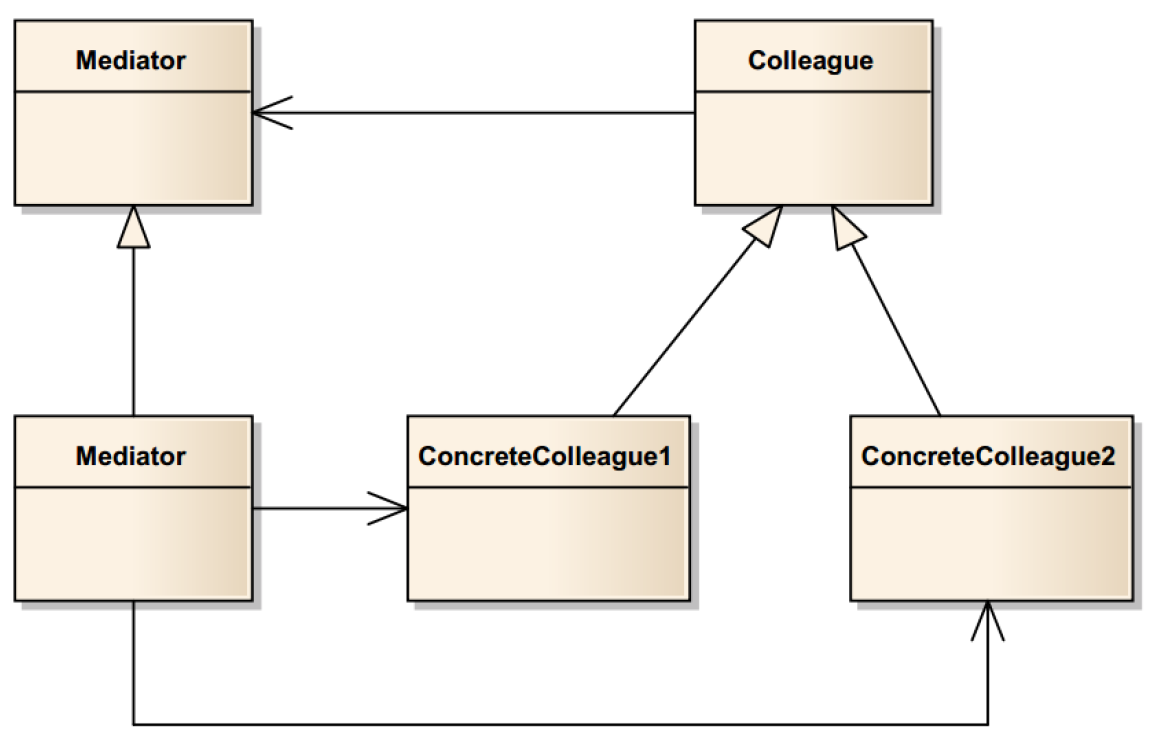
\includegraphics[width=0.7\linewidth]{figs/mediator/mediatorPattern.PNG}
	\caption{Et mediator pattern}
	\label{fig:mediatorPattern}
\end{figure}

\paragraph{Definition af mediators elementer}
\begin{itemize}
	\item BaseMediator\\
	Definerer et interface til kommunikation med "Colleague objekterne".
	\item ConcreteMediator\\
	Imlementerer kommunikationsinterfacet, ved at koordinere Colleague objekter.
	\item Colleague Klasser.
	\begin{itemize}
		\item Hver colleague klasse kender sit mediator object.
		\item Når colleaguen vil snakke med en anden klasse, kommunikeres der udelukkende gennem
		mediatoren.
	\end{itemize}
\end{itemize}

Brugen af et mediator pattern begrænser mængden af afedte klasser i et system, i og med
mediatoren centraliserer funktionalitet der ellers ville være spredt ud på mange klasser. Ved at
pakke objekters interkonnektivitet ind i et mediator pattern, får man samtidig skabt et ekstra
abtraktionsniveau der gør funktionalitet mere overskuelig.

\subsection{Sammenlign de forskellige variationer af GoF Mediator - hvilke bør anvendes hvornår?}

\subsection{Sammenlign de to Design Patterns GoF Observer og GoF Mediator - hvornår vil du anvende hvilket og hvorfor?}

\subsection{Redegør for fordele og ulemper ved anvendelsen af GoF Mediator}

\subsection{Redegør for hvilke(t) SOLID-princip(per) du mener anvendelsen af GoF Mediator understøtter}